Here, we demonstrate the extent to which caching improves mobile PLT.
We also isolate the computational resource that differentiates caching's effect on mobile versus desktop.

\subsection{Workload Characteristics}
We first note several key characteristics of our data corpus:

\textbf{Data Set}. We selected a random subset of 400 of the Alexa top 2000 URLs~\cite{alexa} and loaded their root URL (`/').
% \textbf{Cache Hit Ratio}. We experiment with two settings of cache hit ratio. To show an upper bound on how much caching can help, we evaluate the effect of a perfect (100\%) cache. We also seek to reproduce the result from Flywheel~\cite{flywheel}, by showing the difference between 20\% and 30\% cache hit ratio.
% %In their NSDI paper, Google reported that increasing the cache hit ratio by more than 50\% only increased mobile PLT by 1-2\%. Here, we seek to capture an upper bound on caching's effect on PLT. 

\textbf{Fraction of Cacheable Bytes}. Over 90\% of web pages in our workload have more than 90\% of their total bytes marked as cacheable, as shown in Figure~\ref{fig:cacheable_bytes_linear}. %This gives the initial impression that perfect caching should have a significant effect on web performance.
%Web pages generally make high use of caching between origin servers and users.

\textbf{Total Bytes}. Figure~\ref{fig:total_bytes_linear} shows the spread of web page sizes in our data set. While 95\% of web pages are under 6.8 MB, the median web page size is less than 1.2 MB.

\textbf{Initial Network Delays}. Across all requests/response pairs, the median delay between sending the request and receiving the first response byte was 50ms, with a mean of 151.17ms and standard deviation of 403.77ms.
Initial network delays may play a role in determining the final results of our caching analysis. 
%As such, we experimented with inflating all network delays by a fixed amount (100ms) to emulate what clients in an emerging market might observe. We found that the mobile results of our caching analysis were changed by 3\% in the median case (See Figure~\ref{fig:inflated_delays}).
%\arvind{this is to the original website right?  the "LAN" is confusing.}

\textbf{User Agent}. Many web pages are now optimized for the mobile experience. Web servers inspect the user agents (UA) of incoming HTTP(S) requests to deliver customized content to the client depending on their device size and computational resources. We ran all of our experiments twice: once where the browsers (both desktop and mobile) advertised a mobile UA, and once where the browsers advertised a desktop UA. We found that the differences in their results were comparable and that caching has the same effect on page load time. Here, we show only the desktop UA results to make graphs more readable.
%\arvind{shouldn't it be that the mobile device should use mobile UA and the desktop one should use the desktop UA? the fact that the differences - as opposed to the actual values - are comparable is interesting.} \jamshed{Add slight anecdotal evidence}

\subsection{Performance}
As we saw in Figure~\ref{fig:cacheable_bytes_linear}, most pages are composed of a significant number of cacheable bytes. This would seem to suggest that increasing cache hit ratio should yield a significant improvement in web performance for the end user~\cite{kroeger1997exploring}.

\textbf{Caching Doesn't Significantly Reduce Mobile PLT}.
Similar to Flywheel's result~\cite{flywheel}, we find that increasing the cache hit ratio of a web page does not significantly decrease the user's overall latency on a mobile device.
In fact, with a perfect cache, a mobile device gains only a 13\% PLT reduction in the median case, while its desktop counterpart sees a  PLT reduction of 34\% (see Figure~\ref{fig:percent_reduction_linear}).

Additionally, we emulated partial caches with 20\% and 30\% hit ratios. As shown in Figure~\ref{fig:partial_cache_linear}, we found that increasing the hit ratio by 10 percentage points had negligible effects on mobile page load time. Consistent with Flywheel's NSDI paper, there was only a 1\% reduction in PLT in the median case.

This result is counter-intuitive: for each 10 percentage point increase in cache hit ratio, there is only a 1 percentage point decrease in mobile page load time.
\begin{figure}[t]
    %\hspace{-10pt}
    \figuretitle{Ratio of Fraction Cacheable Bytes to PLT}
    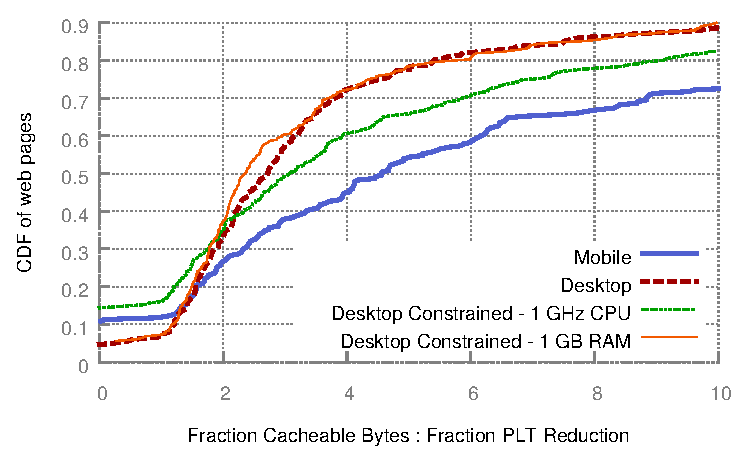
\includegraphics[width=3in]{../graphs/ratio_bytes_to_reduction/ratio_linear_comparison.pdf}
    \caption[]{\label{fig:ratio_linear_comparison}As the percentage of cacheable bytes in a web page increases, the reduction in page load time due to caching increases. However, for each additional percentage cached, there is less than a percentage reduction in page load time.}
\end{figure}
\subsection{Isolating the Difference Between Mobile and Desktop}


% Discuss resource constraints, CPU
We find that the main cause of discrepancy is due to the large difference of CPU speed between desktops and mobile devices. 
We measured this effect by running the same experiment as before, but in virtual machines that were constrained by different resources (using VirtualBox to either set a limit on memory usage or emulate a slower CPU clock speed).
A typical mobile device in the global market today has a 1 GHz processor and 1 GB of RAM~\cite{mobile-stats}. In order to emulate these conditions and isolate computational resources, we restricted one virtual machine to a 1 GHz processor with 6 GB of memory, and another to a 3.2 GHz processor with 1 GB of RAM.

%\colin{Need to also say how much memory/CPU it had, even if if you're focusing on CPU/memory}
In Figure~\ref{fig:percent_reduction_linear}, `Desktop Constrained - 1 GHz CPU' is closely aligned with the results for `Mobile' (our tablet), while `Desktop Constrained - 1 GB RAM' is more closely aligned with the `Desktop' results.
This suggest that CPU is the key difference between caching's effects for mobile and desktop.
In fact, as we throttle CPU constraints, perfect caching has noticeably smaller effects on PLT (See Figure~\ref{fig:plt_cpu_comparison}). Similarly, page load times are generally higher on devices with CPU constraints as seen in Figure~\ref{fig:plt_differences}.

%\colin{Can cut this if we need space}
Consistent with the results found in WProf~\cite{wang2013demystifying}, our results show that reduction in PLT is not proportional to number of bytes cached. We conjecture that the reason mobile performs worse than desktop is precisely because a constrained CPU changes the critical path (when compared to desktop), causing a smaller fraction of the critical path to be network-bound. 
%We hypothesize that the delays of objects on the critical path are also elongated by a constrained CPU.
%These factors contribute to a longer critical path that is prone to the benefits of caching.
%\arvind{above discussion is not clear; and it is probably the most critical observation that we need to communicate precisely}


\subsection{Data Validation}
\label{subsec:validation}
We made several efforts to sanity check the validity our results~\cite{sanity-checks}. 

To mitigate non-determinism, we compared the status codes of all objects loaded in the browser from both original and perfect/partial cache benchmarks. We filtered out about 9\% of web pages in our 400 URL data set in cases where there were a high number of 404 error codes due to non-deterministic requests without responses in the WPR archive. It is worth noting that the figures we present show only these 91\% of web pages that passed this filter.

As the ratio of cached to non-cached bytes increases in a web page, we expect page load time to be strictly less than or equal to that of its non-cached counterpart. As seen in Figure~\ref{fig:ratio_linear_comparison}, there is a positive correlation between the fraction of cached bytes and the reduction in PLT, albeit asymptotic.
However, due to variance in PLT (discussed in \ref{known_limitations}), we see that a fraction of web pages can perform worse when cached, as seen by points to the left of \texttt{X = 0} in Figure~\ref{fig:percent_reduction_linear}.



\begin{figure}[t]
    %\hspace*{-0.11in}
    \figuretitle{CPU Comparison of PLT Reduction}
    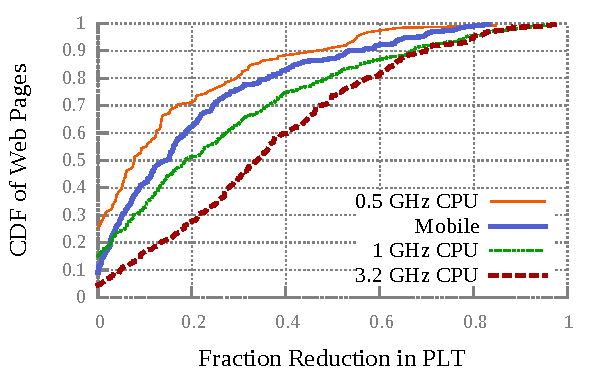
\includegraphics[width=3in]{../graphs/percent_plt_reduction/percent_reduction_linear_CPU_comparison.pdf}
    \caption[]{\label{fig:plt_cpu_comparison}Slower CPU speeds curtail the efficacy of caching to reduce page load time.}
\end{figure}
